%----------createGeneralizationBetweenAssociations----------------------------------------
\op
{createGeneralizationBetweenAssociations}
{Creates a new generalization relationship between two associations}
{createGeneralizationBetweenAssociations(Association selectedEObject,
Association tgt)}
{The association which will become the general element}
{
\begin{itemize}
 \item tgt/targetAssociation: the association which will become the special
 element and inherit from the general element
\end{itemize}
}
{The new generalization relationship must not create an inheritance-cycle (see
\ref{subsec:checkInheritanceCycle})}
{A generalization and references to the input selected association
(the parent) and the target association (the child) are created.} \begin{figure}[H]
  \centering
  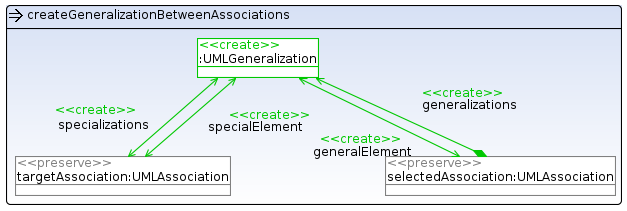
\includegraphics[width=0.8\textwidth]{pics/createGeneralizationBetweenAssociations.png}
  \caption{createGeneralizationBetweenAssociations}
  \label{createGeneralizationBetweenAssociations}
\end{figure}
%----------createGeneralizationBetweenClasses----------------------------------------
\op
{createGeneralizationBetweenClasses}
{Creates a new generalization relationship between classes}
{createGeneralizationBetweenClasses(Class selectedEObject,
Class tgt)}
{The class which will become the general element}
{
\begin{itemize}
 \item tgt/targetClass: the class which will become the special
 element and inherit from the general element
\end{itemize}
}
{The new generalization relationship must not create an inheritance-cycle (see
\ref{subsec:checkInheritanceCycle})}
{A generalization and references to the input selected class
(the parent) and the target class (the child) are created.}
\begin{figure}[H]
  \centering
  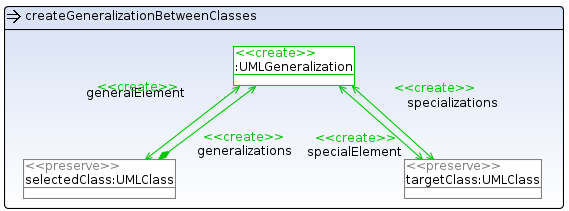
\includegraphics[width=0.8\textwidth]{pics/createGeneralizationBetweenClasses.png}
  \caption{createGeneralizationBetweenClasses}
  \label{createGeneralizationBetweenClasses}
\end{figure}
%----------createGeneralizationBetweenInterfacees----------------------------------------
\op
{createGeneralizationBetweenInterfaces}
{Creates a new generalization relationship between interfaces}
{createGeneralizationBetweenInterfacees(Interface selectedEObject,
Interface tgt)}
{The interface which will become the general element}
{
\begin{itemize}
 \item tgt/targetInterface: the interface which will become the special
 element and inherit from the general element
\end{itemize}
}
{The new generalization relationship must not create an inheritance-cycle (see
\ref{subsec:checkInheritanceCycle})}
{A generalization and references to the input selected interface
(the parent) and the target interface (the child) are created.}
\begin{figure}[H]
  \centering
  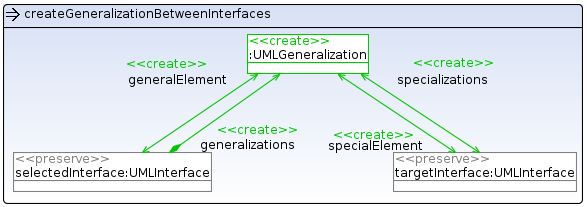
\includegraphics[width=0.8\textwidth]{pics/createGeneralizationBetweenInterfaces.png}
  \caption{createGeneralizationBetweenInterfaces}
  \label{createGeneralizationBetweenInterfaces}
\end{figure}
%----------deleteGeneralizationBetweenAssociations----------------------------------------
\op
{deleteGeneralizationBetweenAssociations}
{Deletes a generalization between associations}
{deleteGeneralizationBetweenAssociations(Generalization selectedEObject)}
{The generalization which should be deleted}
{-}
{-}
{First the references from the associations to the generalization are deleted
and then the selected generalization itself.} \begin{figure}[H]
  \centering
  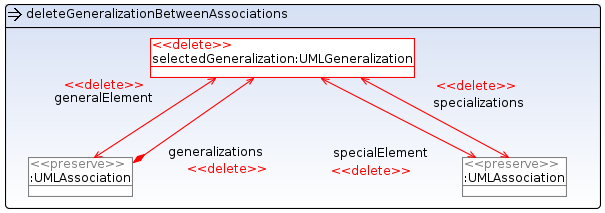
\includegraphics[width=0.8\textwidth]{pics/deleteGeneralizationBetweenAssociations.png}
  \caption{deleteGeneralizationBetweenAssociations}
  \label{deleteGeneralizationBetweenAssociations}
\end{figure}
%----------deleteGeneralizationBetweenAssociations----------------------------------------
\op
{deleteGeneralizationBetweenClasses}
{Deletes a generalization between classes}
{deleteGeneralizationBetweenClasses(Generalization selectedEObject)}
{The generalization which should be deleted}
{-}
{-}
{First the references from the classes to the generalization are deleted
and then the selected generalization itself.}
\begin{figure}[H]
  \centering
  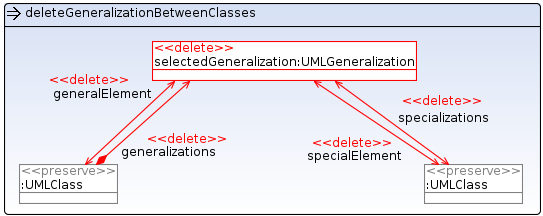
\includegraphics[width=0.8\textwidth]{pics/deleteGeneralizationBetweenClasses.png}
  \caption{deleteGeneralizationBetweenClasses}
  \label{deleteGeneralizationBetweenClasses}
\end{figure}
%----------deleteGeneralizationBetweenInterfaces----------------------------------------
\op
{deleteGeneralizationBetweenInterfaces}
{Deletes a generalization between interfaces}
{deleteGeneralizationBetweenInterfaces(Generalization selectedEObject)}
{The generalization which should be deleted}
{-}
{-}
{First the references from the interfaces to the generalization are deleted
and then the selected generalization itself.}
\begin{figure}[H]
  \centering
  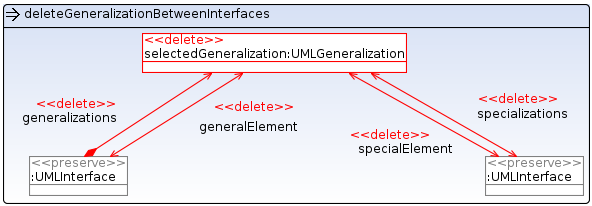
\includegraphics[width=0.8\textwidth]{pics/deleteGeneralizationBetweenInterfaces.png}
  \caption{deleteGeneralizationBetweenInterfaces}
  \label{deleteGeneralizationBetweenInterfaces}
\end{figure}
%----------editGeneralizationGeneralElementFromAssociationToAssociation----------------------------------------
\op
{editGeneralizationGeneralElementFromAssociationToAssociation}
{Replaces the general element of a generalization from an association by
another}
{editGeneralizationGeneralElementFromAssociationToAssociation(Generalization
selectedEObject, Association src, Association tgt)}
{The generalization whose general element should be changed.} {
\begin{itemize}
 \item src/oldAssociation: The old association as general element
 \item tgt/newAssociation: The new association as general element
\end{itemize}
}
{The new generalization relationship must not create an inheritance-cycle (see
\ref{subsec:checkInheritanceCycle})}
{Only references change.}
\begin{figure}[H]
  \centering
  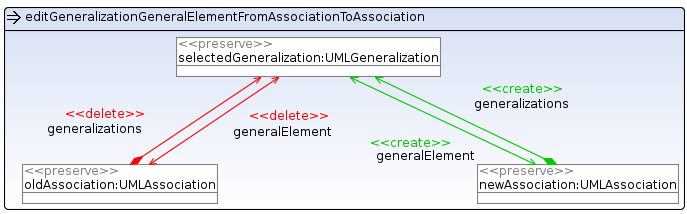
\includegraphics[width=1.0\textwidth]{pics/editGeneralizationGeneralElementFromAssociationToAssociation.png}
  \caption{editGeneralizationGeneralElementFromAssociationToAssociation}
  \label{editGeneralizationGeneralElementFromAssociationToAssociation}
\end{figure}
%----------editGeneralizationGeneralElementFromClassToClass----------------------------------------
\op
{editGeneralizationGeneralElementFromClassToClass}
{Replaces the general element of a generalization from an class by
another}
{editGeneralizationGeneralElementFromClassToClass(Generalization
selectedEObject, Class src, Class tgt)}
{The generalization whose general element should be changed.} {
\begin{itemize}
 \item src/oldClass: The old class as general element
 \item tgt/newClass: The new class as general element
\end{itemize}
}
{The new generalization relationship must not create an inheritance-cycle (see
\ref{subsec:checkInheritanceCycle})}
{Only references change.}
\begin{figure}[H]
  \centering
  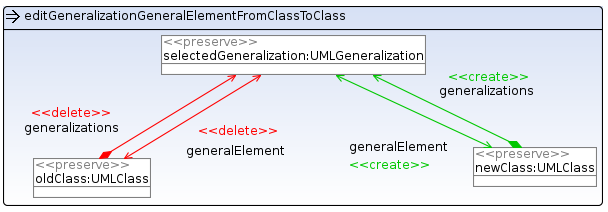
\includegraphics[width=1.0\textwidth]{pics/editGeneralizationGeneralElementFromClassToClass.png}
  \caption{editGeneralizationGeneralElementFromClassToClass}
  \label{editGeneralizationGeneralElementFromClassToClass}
\end{figure}
%----------editGeneralizationGeneralElementFromInterfaceToInterface----------------------------------------
\op
{editGeneralizationGeneralElementFromInterfaceToInterface}
{Replaces the general element of a generalization from an interface by
another}
{editGeneralizationGeneralElementFromInterfaceToInterface(Generalization
selectedEObject, Interface src, Interface tgt)}
{The generalization whose general element should be changed.} {
\begin{itemize}
 \item src/oldInterface: The old interface as general element
 \item tgt/newInterface: The new interface as general element
\end{itemize}
}
{The new generalization relationship must not create an inheritance-cycle (see
\ref{subsec:checkInheritanceCycle})}
{Only references change.}
\begin{figure}[H]
  \centering
  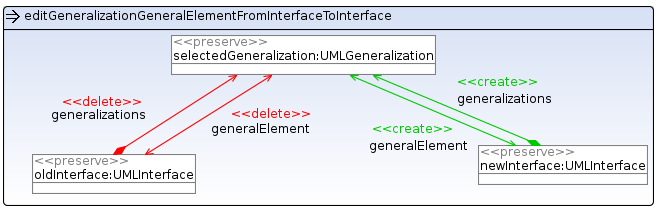
\includegraphics[width=1.0\textwidth]{pics/editGeneralizationGeneralElementFromInterfaceToInterface.png}
  \caption{editGeneralizationGeneralElementFromInterfaceToInterface}
  \label{editGeneralizationGeneralElementFromInterfaceToInterface}
\end{figure}
%----------editGeneralizationSpecialElementFromInterfaceToInterface----------------------------------------
\op
{editGeneralizationSpecialElementFromInterfaceToInterface}
{Edits the special element of a specialization from an interface to
another}
{editGeneralizationSpecialElementFromInterfaceToInterface(Generalization
selectedEObject, Interface src, Interface tgt)}
{The specialization whose special element should be changed.} {
\begin{itemize}
 \item src/oldInterface: The old interface as special element
 \item tgt/newInterface: The new interface as special element
\end{itemize}
}
{The new generalization relationship must not create an inheritance-cycle (see
\ref{subsec:checkInheritanceCycle})}
{Only references change.}
\begin{figure}[H]
  \centering
  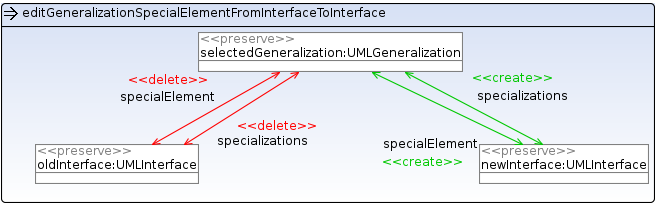
\includegraphics[width=1.0\textwidth]{pics/editGeneralizationSpecialElementFromInterfaceToInterface.png}
  \caption{editGeneralizationSpecialElementFromInterfaceToInterface}
  \label{editGeneralizationSpecialElementFromInterfaceToInterface}
\end{figure}
%----------editGeneralizationSpecialElementFromClassToClass----------------------------------------
\op
{editGeneralizationSpecialElementFromClassToClass}
{Edits the special element of a specialization from an class to
another}
{editGeneralizationSpecialElementFromClassToClass(Generalization
selectedEObject, Class src, Class tgt)}
{The specialization whose special element should be changed.} {
\begin{itemize}
 \item src/oldClass: The old class as special element
 \item tgt/newClass: The new class as special element
\end{itemize}
}
{The new generalization relationship must not create an inheritance-cycle (see
\ref{subsec:checkInheritanceCycle})}
{Only references change.}
\begin{figure}[H]
  \centering
  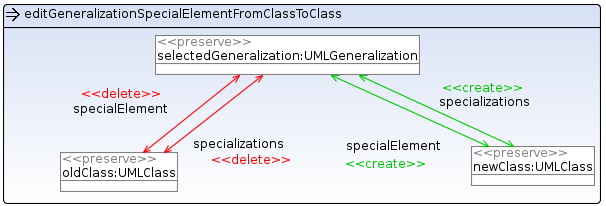
\includegraphics[width=1.0\textwidth]{pics/editGeneralizationSpecialElementFromClassToClass.png}
  \caption{editGeneralizationSpecialElementFromClassToClass}
  \label{editGeneralizationSpecialElementFromClassToClass}
\end{figure}
%----------editGeneralizationSpecialElementFromAssociationToAssociation----------------------------------------
\op
{editGeneralizationSpecialElementFromAssociationToAssociation}
{Edits the special element of a specialization from an association to
another}
{editGeneralizationSpecialElementFromAssociationToAssociation(Generalization
selectedEObject, Association src, Association tgt)}
{The specialization whose special element should be changed.} {
\begin{itemize}
 \item src/oldAssociation: The old association as special element
 \item tgt/newAssociation: The new association as special element
\end{itemize}
}
{The new generalization relationship must not create an inheritance-cycle (see
\ref{subsec:checkInheritanceCycle})}
{Only references change.}
\begin{figure}[H]
  \centering
  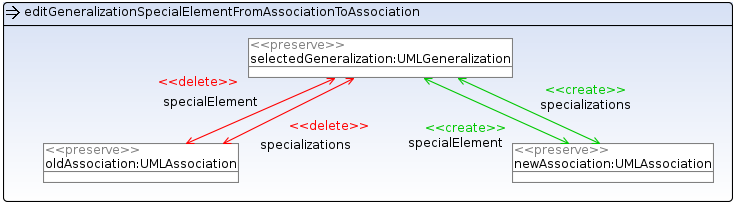
\includegraphics[width=1.0\textwidth]{pics/editGeneralizationSpecialElementFromAssociationToAssociation.png}
  \caption{editGeneralizationSpecialElementFromAssociationToAssociation}
  \label{editGeneralizationSpecialElementFromAssociationToAssociation}
\end{figure}
